\documentclass{article}
\usepackage{amsmath, amssymb}
\usepackage[retainorgcmds]{IEEEtrantools}
\usepackage{filecontents}
\usepackage{hyperref}
\usepackage{algpseudocode}
\usepackage{graphicx}
\author{Derek Kuo, Henry Milner}
\title{CS267 HW3}
\date{04/03/15}

% Some functions for general use.

\def\seqn#1\eeqn{\begin{align}#1\end{align}}

\newcommand{\vecName}[1]%
  {\boldsymbol{#1}}

\newcommand{\io}%
  {\text{ i.o. }}

\newcommand{\eventually}%
  {\text{ eventually }}

\newcommand{\tr}%
  {\text{tr}}

\newcommand{\Cov}%
  {\text{Cov}}

\newcommand{\adj}%
  {\text{adj}}

\newcommand{\funcName}[1]%
  {\text{#1}}

\newcommand{\hasDist}%
  {\sim}

\DeclareMathOperator*{\E}%
  {\mathbb{E}}

\newcommand{\Var}%
  {\text{Var}}

\newcommand{\std}%
  {\text{std}}

\newcommand{\grad}%
  {\nabla}

\DeclareMathOperator*{\argmin}{arg\,min}

\DeclareMathOperator*{\argmax}{arg\,max}

\newcommand{\inprod}[2]%
  {\langle #1, #2 \rangle}

\newcommand{\dd}[1]%
  {\frac{\delta}{\delta#1}}

\newcommand{\Reals}%
  {\mathbb{R}}

\newcommand{\indep}%
  {\protect\mathpalette{\protect\independenT}{\perp}} \def\independenT#1#2{\mathrel{\rlap{$#1#2$}\mkern2mu{#1#2}}}

\newcommand{\defeq}%
  {\buildrel\triangle\over =}

\newcommand{\defn}[1]%
  {\emph{Definition: #1}\\}

\newcommand{\example}[1]%
  {\emph{Example: #1}\\}

\newcommand{\figref}[1]%
  {\figurename~\ref{#1}}

\newtheorem{theorem}{Theorem}[section]
\newtheorem{lemma}[theorem]{Lemma}
\newenvironment{proof}[1][Proof]{\begin{trivlist}
\item[\hskip \labelsep {\bfseries #1}]}{\end{trivlist}}

\begin{filecontents}{\jobname.bib}
@inproceedings{shet2009asynchronous,
  title={Asynchronous programming in UPC: A case study and potential for improvement},
  author={Shet, Aniruddha and Tipparaju, Vinod and Harrison, Robert},
  organization={Citeseer}
}
@inproceedings{wang2011exploiting,
  title={Exploiting Hierarchical Parallelism Using UPC},
  author={Wang, Lingyuan and Merchant, Saumil and El-Ghazawi, Tarek},
  booktitle={Parallel and Distributed Processing Workshops and Phd Forum (IPDPSW), 2011 IEEE International Symposium on},
  pages={1216--1224},
  year={2011},
  organization={IEEE}
}
\end{filecontents}

\begin{document}
\maketitle

\section{Introduction}
We first describe our implementation of distributed contig generation in UPC.  Then, we present some information about the performance and scaling properties of our implementation.  Finally, we offer some comments.

\subsection{Notation}
We use $P$ to denote the number of processors used in a computation.  We use $n$ to denote the number of kmers in a workload.  $H$ denotes the size of the hash table we use to store the kmers, which is always a multiple of $P$ (in fact it is equal to $P \operatorname{ceil}(n/P)$ in our experiments).  The hash value of a kmer is a number in the set $[H]$.  The ``local hash value'' of a kmer is its hash value modulo $H/P$.  The ``destination processor'' of a kmer is its hash value module $P$.

\section{Implementation}
A parallel implementation of contig generation is useful only for handling large genomes that grow with the problem size.  If we are sequencing genomes of a small fixed size, we have an embarrassingly parallel problem to which serial code is likely better suited.  So, when there are design choices to be made, we will target the large-genome regime.

\subsection{Graph Creation}
The hard part of graph creation is just a distributed hash-based shuffle, like the shuffle stage in a MapReduce job.  This involves all-to-all communication of approximately $1-1/P$ of the data.  Importantly, viewing graph creation as a hash shuffle means that we can a very small number of communication rounds, incurring network latency costs of only $O(P)$ rounds per processor and, as we will see, entirely avoiding the use of locks.

We partition the hash space evenly among processors, with processor $i$ receiving all kmers with hash value $\{iH/P, iH/P+1, \cdots, (i+1)H/P-1\}$.  Each processor reads a portion of the input file, then hashes each kmer to determine its destination processor.  Each processor writes the number of kmers it will send to each other processor (including itself), using a shared array of size $P^2$.  Then, for each processor $i$, for each other processor $j$, processor $i$ allocates a shared array with local affinity (a \texttt{shared [] kmer\_t *}, which we call a ``send buffer'') and places the kmers read on $i$ with destination processor $j$ in that send buffer.  (Shared pointers to these send buffers are placed in a shared array of size $P^2$.)  A single barrier at this point ensures that all the send buffers (and their sizes) have been filled in.  Then, each processor allocates a private buffer to receive kmers from each other processor, and reads from the send buffers.

After each kmer has been shuffled to the appropriate machine, graph creation is embarrassingly parallel.  We create a shared array for the hash table, which is a \texttt{shared [1] shared\_kmer\_bucket\_t *} of size equal to the hash table size, where \texttt{shared\_kmer\_bucket\_t} is a \texttt{shared [] kmer\_t *}.  A kmer with destination processor $j$ and local hash value $h$ will reside in bucket $hP+j$ in this shared array.  Buckets are implemented as flat arrays; there is an additional shared array, a \texttt{shared [1] int *} of size equal to the hash table size, called a bucket-size table, to store the size of each bucket.  We first insert all the local kmers into temporary buckets that are private dynamic arrays, then allocate each bucket in shared memory with an appropriate size (with local affinity) and store its pointer in the shared hash table and its size in the shared bucket-size table.  Another barrier ensures that the hash table has been filled in before graph traversal begins.

In this scheme, a lookup in the hash table involves a lookup in the bucket-size table, a lookup in the hash table for a pointer to the bucket, and a \texttt{upc\_memget} to fetch the bucket, which is of expected size $1$ (and maximum size $O(\log n / \log \log n)$ with high probability).  In our implementation, each of these steps is done serially, so there are $3$ rounds of communication for every lookup.

A few final notes on graph creation:
\begin{enumerate}
  \item Only two synchronization steps are required -- one to ensure that each thread has finished writing to its send buffers, and another to ensure that each thread has finished writing its part of the hash table.  We use no locks or atomic operations.
  \item All communication is done using packed kmers.  A packed kmer uses 2 bits per base pair, plus a byte to store its forward and backward extensions (which may be the usual nucleotides or the indicator for the start of a contig).
  \item It is possible in principle to pipeline the communication stage of the hash shuffle -- that is, each processor could communicate with each other processor simultaneously.  With full bisection bandwidth this would dramatically speed up the communication stage.  However, the version of UPC we are using does not seem to support asynchronous remote reads, so each processor must communicate serially with each other processor in our implementation.  Apparently there is some work on extending UPC to allow asynchronous remote communication \cite{shet2009asynchronous}.
\end{enumerate}

\subsection{Graph Traversal}
Graph traversal is straightforward.  Each machine filters its own kmers to find those with an \'F\' backward extension.  Then, for each machine (in parallel), for each kmer in the start list, we traverse the graph until we reach a kmer with an \'F\' forward extension.  Since we are guaranteed that we start at the end of a connected component that is a chain, traversing the graph is simply traversing a linked list.  Given that the last $K$ nucleotides of the current contig (including the last forward extension) are string $x$, we look up $x$ in the hash table.  The forward extension of that string gives us one nucleotide to extend the contig, or tells us we are done with the contig.  Each step involves (as noted above) 3 rounds of communication, except in the rare case that $x$ happens to reside on the same processor as the start kmer.  Each processor blocks while waiting for the next forward extension to be fetched.

\section{Results}
\subsection{Small experiment}

\begin{figure}
  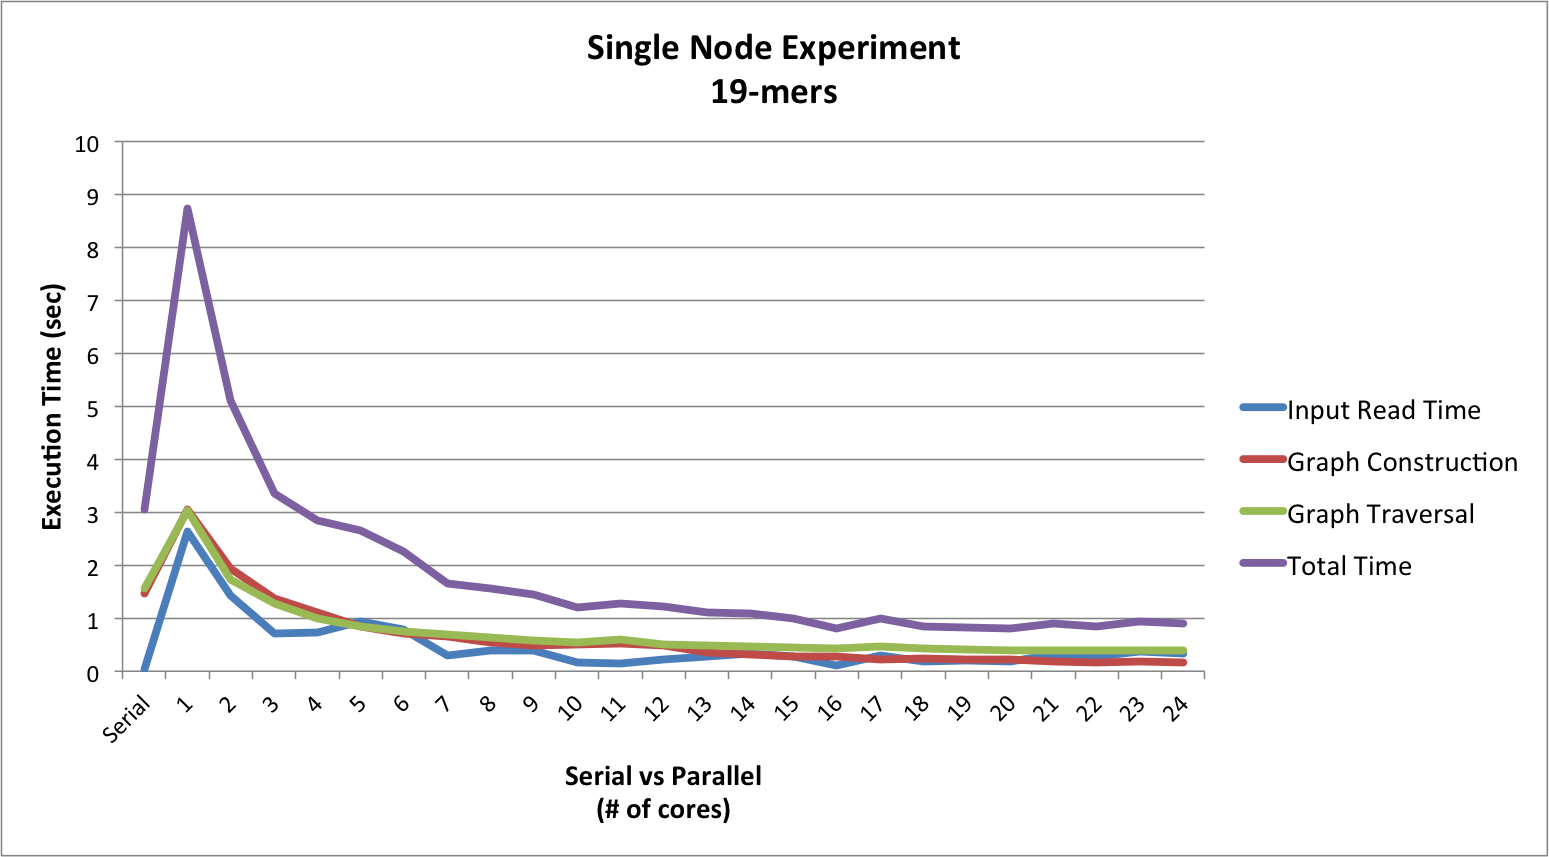
\includegraphics[width=\textwidth]{plots/Result_single_small.png}
  \caption{Comparison of serial and parallel algorithms on small input (19-mers).}
  \label{fig:small}
\end{figure}

Figure \ref{fig:small} displays results for the small 19-mers input.  Both graph construction and graph traversal perform worse than the serial code when given only a few cores ($P<3$); this indicates that there is substantial constant overhead in the parallel code.  With more cores, both construction and traversal time decrease, and the parallel code eventually beats the serial code.  Graph construction exhibits (approximately) strong scaling, but graph traversal improves more slowly with $P$.

\subsection{Large experiment}

\begin{figure}
  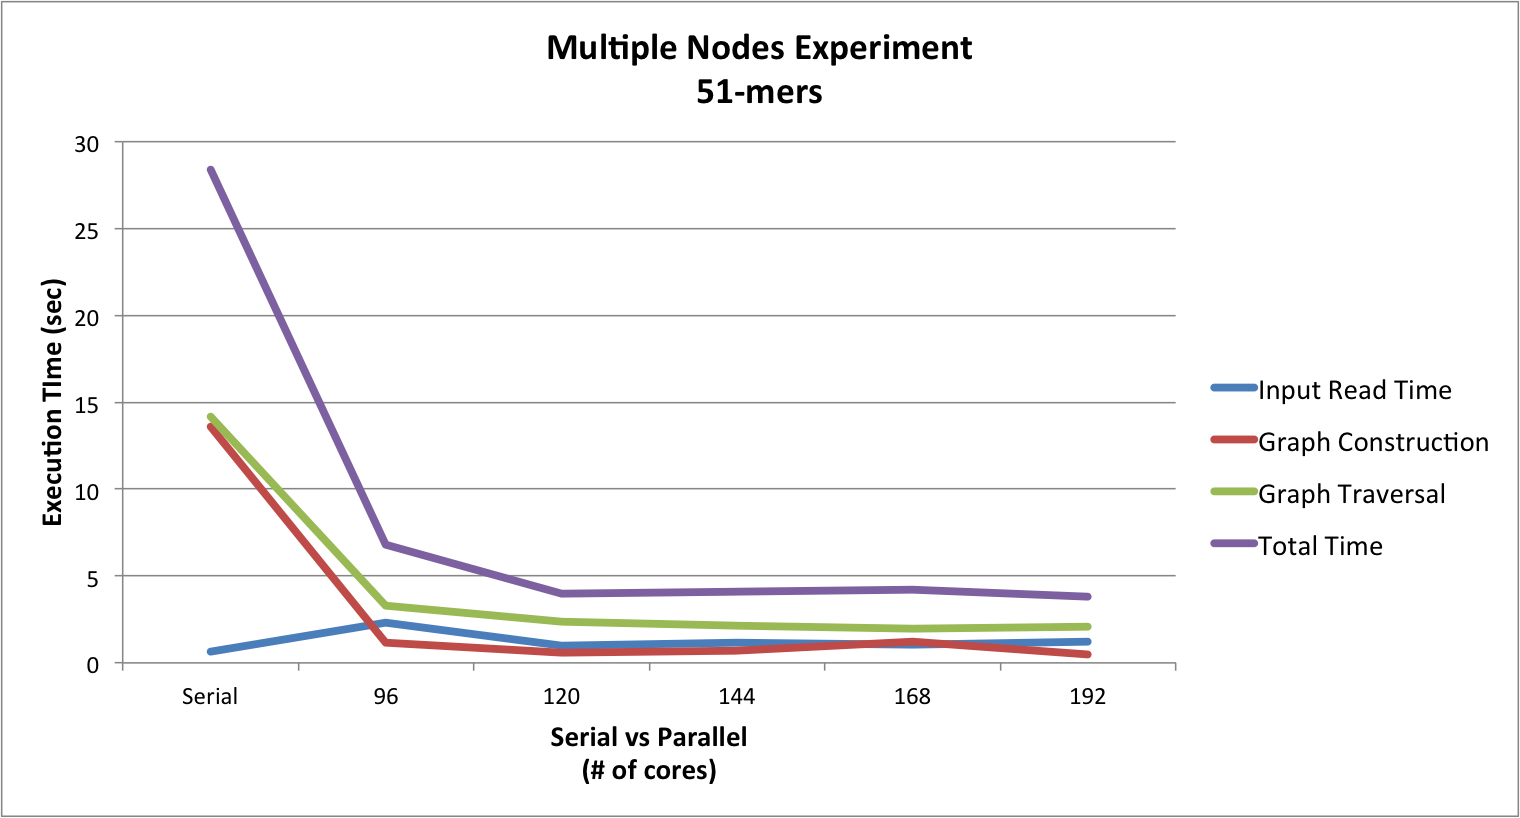
\includegraphics[width=\textwidth]{plots/Result_multiple_large.png}
  \caption{Comparison of serial and parallel algorithms on large input (51-mers).}
  \label{fig:large}
\end{figure}

Figure \ref{fig:large} displays results for the larger 51-mers input.  The performance gap between the serial and parallel versions is wider here, indicating (in a very rough sense) that the parallel version exhibits weak scaling.  For $4$ or more $24$-core nodes ($P=96,120,144,168,$ and $192$), the parallel algorithm is at least 10 times faster on graph construction and 5 times faster on graph traversal.  Performance does not improve significantly with more than $120$ cores, and graph traversal takes about $2$ seconds with that level of parallelism.

A rough calculation shows that the traversal phase should take at least $.35$ seconds for our algorithm: The longest contig has $20711$ nucleotides, network latency on for Hopper's Gemini network is about $3 \mu s$, each nucleotide lookup takes $3$ network round trips, and $(20711-51)*3*2*3*10^{-6} \approxeq .35$.  So we cannot expect to improve much on this performance with our algorithm.

\section{Discussion}
\subsection{Using UPC}
Programming with UPC for the first time was a surprisingly poor experience.  Our list of grievances is:
\begin{description}
  \item[No dynamic block size:] When using \texttt{upc\_all\_alloc}, it is never correct to use a block size that cannot be determined at compilation time, since the block size of the resulting pointer is a compile-time constant.  The UPC documentation never explicitly mentions this.
  \item[Misleading return type of \texttt{upc\_alloc}:] \texttt{upc\_alloc} returns a \texttt{shared void *}, but it is never correct to use it without casting it to a \texttt{shared [] void *}, since it has local affinity.  The UPC documentation never mentions this.
  \item[Poor standards support:] BUPC does not even support the C99 standard.  In particular, we would have liked to have support for dynamic-sized arrays on the stack.
  \item[Cryptic error messages:] Misuse of a shared pointer (see below) would result in a floating point exception in PGAS.  It would have been helpful to get a message like: ``This exception probably resulted from misuse of a shared pointer.''
  \item[Unclear semantics of private-pointer-to-shared:] We at first attempted to use the following scheme for our shared hash table: Each bucket was a linked list head, a struct holding both a kmer and a pointer to the next kmer (that is, a \emph{private} pointer into a \texttt{shared [] kmer\_t} on the machine owning the bucket).  Dereferencing the pointer on another machine did not work and resulted in a FPE.  In a rush to finish the project in time, we gave up on the linked-list scheme.  In retrospect, the problem was probably that we did not declare the pointer itself as shared within the linked list struct.  However, it was not clear to us from the documentation that a private pointer-to-shared would not function properly if used on another processor.
  \item[No support for asynchronous remote communication:] As noted elsewhere in this report, this slowed down our algorithm somewhat.
  \item[Required use of statics:] Statics make functional style impossible and make code more difficult to reason about.  Forgetting that shared objects must be stored in static fields, we at first attempted to use functional style.  It would have been helpful if the compiler had warned us about this; for example, it could have issued a warning when we incorrectly returned a pointer-to-shared from a function.
\end{description}

Some of these issues will be less painful if we use UPC a second time.  Many of our problems stemmed from thinking of UPC as providing an almost-shared memory abstraction.  Given the large number of gotchas in dealing with shared memory, we think the value of UPC is in abstracting away the details of communication; the programmer must still be quite aware of data locality, even at the level of code syntax.

\subsection{An Implementation with Two-Sided Communication}
Implementing graph creation in MPI would not be much different than implementing it in UPC, except that we would have to use explicit calls to \texttt{MPI\_Rput} or \texttt{MPI\_Rget} rather than array accesses in some cases.

Graph traversal would be trickier, but not very hard.  Each processor would send \texttt{MPI\_Rget} requests to the appropriate processors for kmer lookups (one for each contig being processed on the processor), then \texttt{MPI\_Waitany} in a while-loop waiting for these requests to be fulfilled.  When a request is fulfilled, the next \texttt{MPI\_Rget} can be issued.

\subsection{Alternative Algorithms}
Our implementation of graph creation seems close to optimal, given the requirement that the graph be partitioned among all available processors.  However, it is not clear that we have the right overall approach to contig generation.  The dominant cost of contig generation, under our algorithm, is network latency in the traversal phase, and either eliminating or batching communication could greatly improve this.  We have two proposals for that:

\begin{enumerate}
  \item If each processor (or at least each machine) has a local copy of the graph, and the number of contigs is large, the problem is embarrassingly parallel; the shared memory is only read during the traversal, never modified.  The only reason to introduce network communication into the algorithm is that the graph cannot fit into local memory that supports random accesses faster than network communication.  Random access latency for HDDs is typically higher than network latency on a supercomputer.  But using SSDs to store the entire graph on every machine (for example, Amazon EC2's \texttt{i2.8xlarge} instances) could be a superior alternative.  If the data were initially distributed across machines, it would be important to use an efficient broadcast algorithm to initially send every kmer to every machine.
  \item Under the algorithm we have implemented, during graph traversal, each processor iterates through its list of start kmers serially, and blocks while waiting for the next extension in the current contig to be fetched.  Therefore the total depth of network round-trips paid on a processor is $O(\sum_i S_i)$, where $S_i$ is the length of the $i$th contig and the sum is taken over the contigs generated on the processor.  Generating a single contig is difficult to parallelize, though speculative execution, i.e. prefetching many possible extensions of the current kmer, could allow us to pipeline single-contig generation (at least until bandwidth or computation became bottlenecks).  But generating all the contigs on a processor in parallel would allow us to pay only $O(\max_i S_i)$ in depth of network round-trips per machine, under the reasonable assumption that computation and bandwidth are unbounded during the graph traversal phase.  Unfortunately, UPC does not (to our knowledge) support hierarchical multithreading within a single UPC process, though there is research work in that direction \cite{wang2011exploiting}.  Support for asynchronous remote communication would also allow us to implement this approach in UPC.
\end{enumerate}

\subsection{Alternative Problems}
The contig generation problem we have been given is unrealistically easy in many ways.  Let us consider two harder versions of the problem:

\begin{enumerate}
  \item There are $P$ contigs, and their lengths follow a power-law distribution.
  \item There is only a single contig.
\end{enumerate}

It is useful to think of version 2 as an extreme case of version 1, and focus on solving version 2.  The issue with version 2 is that the depth of computation in the graph traversal phase is simply the length of the contig, which is $O(n)$.  (In version 1 of the problem, the expected depth could be made arbitrarily close to $n$.)  Our algorithm might still be better than a serial algorithm if the graph cannot fit in memory, but it will not take advantage of parallel computation.

To handle a long contig, we could use the approach suggested in class: Each processor starts at a random kmer and grows in both directions in arbitrary order.  The challenge is to stitch together the work of different processors without too much overlap.  Here is a simple algorithm: When processor $i$ reads a kmer, it atomically marks it as owned by processor $i$.  (If each kmer resides on only 1 processor, this atomic operation need not involve any network communication.)  When another processor attempts to read a kmer that has already been marked, it stops working in that direction.  Once all processors are done, we find the endpoints of each processor's subcontig and send each subcontig to one machine to be stitched together.

\bibliographystyle{plain}
\bibliography{\jobname}

\end{document}